\section{点列收敛与完备性}
\label{sec:metric-convergence-completeness}

实数列$a_n\to a$的含义是误差$|a_n-a|$趋于零。把绝对值换成一般距离，就得到度量空间中的收敛。但这只回答了一类问题：已经有一个候选极限，检查点列是否逼近它。迭代求解、逐次逼近等问题往往事先不知道极限在哪里，只能观察点列内部的项是否越来越接近。本节先建立收敛和它与闭集的关系，再研究后一类问题，并说明怎样把缺失的极限补进空间。

\subsection{点列的收敛}
\label{sec:metric-convergence}

\begin{definition}[点列的收敛]
\label{def:metric-convergence}
设$(x_n)$是$X$中的点列，$x\in X$。若$d(x_n,x)\to0$，即对任意$\varepsilon>0$存在$N$使$n\geq N$时$d(x_n,x)<\varepsilon$，就称$(x_n)$\term{收敛}（converge）到$x$，记作$x_n\to x$，称$x$为它的极限。
\end{definition}

用开球的语言说，$x_n\to x$表示无论球$B(x,\varepsilon)$多小，点列从某项起都留在球中。实数列的情形见\BookChapterRef{chap:limits-continuity}{卷一“极限与连续”章}，那里的误差$|a_n-a|$在这里换成了$d(x_n,x)$。定义要求极限$x$属于当前空间$X$；如果所谓的极限在$X$之外，那么在$X$中这一列不收敛。

\paragraph{极限的基本性质}
三条基本性质都由三角不等式得到，区别在于各自控制的量。第一，极限唯一：若$x_n\to x$且$x_n\to y$，则$0\leq d(x,y)\leq d(x,x_n)+d(x_n,y)\to0$，故$d(x,y)=0$，$x=y$。第二，收敛列有界：取$\varepsilon=1$得到$N$，则对任意$n$，$d(x_n,x)\leq\max\{1,d(x_1,x),\dots,d(x_{N-1},x)\}$，所有项都落在以$x$为中心的一个有限半径球内。第三，子列保持原极限：若$n_1<n_2<\cdots$，则$n_k\geq k$，所以$k\geq N$时$d(x_{n_k},x)<\varepsilon$。

\paragraph{有限乘积中的收敛}
在有限乘积$X=X_1\times\cdots\times X_m$上取乘积度量$\rho_\infty$或$\rho_1$。由式~\eqref{eq:metric-product-bounds}，$d_i(x_{n,i},x_i)\leq\rho_\infty(x_n,x)\leq\rho_1(x_n,x)\leq\sum_{i=1}^md_i(x_{n,i},x_i)$，其中$x_{n,i}$表示$x_n$的第$i$个坐标。左边的不等式说明整体收敛推出每个坐标收敛；右边的不等式说明各坐标收敛时，有限个趋于零的数之和也趋于零，从而整体收敛。所以在有限乘积中，整体收敛与逐坐标收敛等价，且与选$\rho_1$还是$\rho_\infty$无关。$\mathbb R^d$上$d_1$与$d_\infty$下的收敛都等价于逐坐标收敛；由$d_\infty\leq d_2\leq d_1$，$d_2$下的收敛也是如此。

\paragraph{极限可能不在当前空间中}
取子空间$X=(0,1)$与点列$x_n=1/(n+1)$。在环境空间$\mathbb R$中，$x_n\to0$；但$0\notin X$，而极限唯一，所以$(x_n)$在$X$中没有极限。点列本身没有改变，改变的是允许作为极限的点。

\subsection{闭包与闭集的序列判据}
\label{sec:metric-sequential-closure}

闭包用“每个球都碰到集合”定义，这是关于所有半径的条件。点列把这些半径排成一列$1/n$，于是闭包点可以用集合内的点逐项逼近。

\begin{lemma}[闭包的序列判据]
\label{lem:metric-sequential-closure}
设$A\subseteq X$。则$x\in\overline A$当且仅当存在$A$中的点列$(a_n)$使$a_n\to x$。
\end{lemma}

\begin{proof}
设$x\in\overline A$。对每个$n$，球$B(x,1/n)$与$A$相交，从中取一点$a_n$，则$d(a_n,x)<1/n\to0$。反过来，设$a_n\in A$且$a_n\to x$。对任意$r>0$，存在$n$使$d(a_n,x)<r$，即$a_n\in B(x,r)\cap A$，所以每个球都与$A$相交，$x\in\overline A$。
\end{proof}

由第~\ref{sec:metric-closure}小节，$A$闭当且仅当$\overline A\subseteq A$。结合引理~\ref{lem:metric-sequential-closure}，得到闭集的序列判据：$A$是闭集，当且仅当$A$中的点列只要在$X$中收敛，其极限就属于$A$。例如$[0,1]$在$\mathbb R$中闭，而$(0,1]$不闭，因为$1/n\in(0,1]$收敛到$0\notin(0,1]$。

这个判据只承诺保留已经存在的极限，并不保证点列有极限。$\mathbb Q$在$\mathbb Q$自身中是闭集（全空间总是闭的），但下面会看到，$\mathbb Q$中有项彼此越来越近却没有极限的点列。要讨论极限的存在，需要一个不预先指定候选极限的判据。

\subsection{柯西列与完备性}
\label{sec:metric-cauchy}

用逐次逼近求解时，我们只能看到已经算出的项。若从某项起任意两项都足够接近，就有理由期望点列趋于某个极限；但这需要空间里确实有那个极限。

\begin{definition}[柯西列与完备空间]
\label{def:metric-complete}
若对任意$\varepsilon>0$存在$N$，使$m,n\geq N$时$d(x_m,x_n)<\varepsilon$，就称$(x_n)$为\term{柯西列}（Cauchy sequence）。若$X$中的每个柯西列都收敛到$X$中的某点，就称$(X,d)$是\term{完备}（complete）的，也称完备度量空间。
\end{definition}

柯西条件只涉及点列自身的项，不涉及任何候选极限。收敛列一定是柯西列：若$x_n\to x$，对$\varepsilon>0$取$N$使$n\geq N$时$d(x_n,x)<\varepsilon/2$，则$m,n\geq N$时$d(x_m,x_n)\leq d(x_m,x)+d(x,x_n)<\varepsilon$。反过来不一定成立，结论取决于空间。

\begin{example}[有理数中不收敛的柯西列]
\label{ex:metric-rational-cauchy}
令$q_n$为$\sqrt2$的十进制展开截到小数点后第$n$位，即$q_0=1$、$q_1=1.4$、$q_2=1.41$、$q_3=1.414$、$q_4=1.4142$，以此类推。每个$q_n$都是有理数，并且$q_n\leq\sqrt2<q_n+10^{-n}$。当$m\geq n$时，$q_m$与$q_n$的前$n$位相同，所以$0\leq q_m-q_n<10^{-n}$，$(q_n)$是$\mathbb Q$中（通常距离下）的柯西列。在$\mathbb R$中$q_n\to\sqrt2$，而$\sqrt2$是无理数；由极限唯一性，$(q_n)$在$\mathbb Q$中没有极限。所以$\mathbb Q$不完备。图~\ref{fig:metric-rational-cauchy}画出了这些项向$\sqrt2$处的“空缺”聚拢的情形。
\end{example}

\begin{figure}[!htbp]
  \centering
  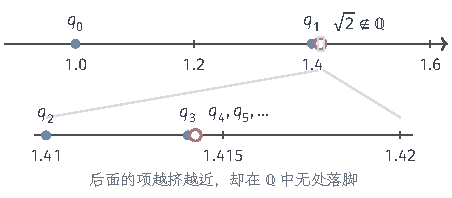
\includegraphics[width=76.616mm]{figures/02-abstract-mathematics/01-metric-and-measure/tikz/c1-rational-cauchy/figure.pdf}
  \caption{有理数中不收敛的柯西列。上方数轴上的蓝点是$\sqrt2$的十进制截断$1,\ 1.4,\ 1.41,\ 1.414$，空心圆标出$\sqrt2\approx1.41421$，它不属于$\mathbb Q$；下方放大$[1.41,1.42]$一段，可见后面的项继续向空心圆聚拢。从第$n$项起任意两项相差不到$10^{-n}$，但在$\mathbb Q$中找不到它们的极限。}
  \label{fig:metric-rational-cauchy}
\end{figure}

\paragraph{实数与欧氏空间的完备性}
实数在通常距离下是完备的，这正是卷一“极限与连续”章中的柯西收敛准则，它依赖实数的确界性质。由此可以得到$\mathbb R^d$的完备性：若$(\bm x_n)$在$d_2$下是柯西列，由$|x_{m,i}-x_{n,i}|\leq d_2(\bm x_m,\bm x_n)$，每个坐标都是实数柯西列，各自收敛到某个$x_i$；令$\bm x=(x_1,\dots,x_d)$，由上一小节，逐坐标收敛推出$d_2(\bm x_n,\bm x)\to0$。同样的论证适用于$d_1$与$d_\infty$。

\paragraph{完备子集与闭子集}
完备性与闭性之间有两个方向不同的结论，前者需要环境空间完备，后者对任意度量空间成立。

\begin{theorem}[完备性与闭集]
\label{thm:metric-complete-closed}
设$A\subseteq X$配备子空间度量。
\begin{enumerate}
  \item 若$X$完备且$A$在$X$中闭，则$A$完备。
  \item 若$A$完备，则$A$在$X$中闭。
\end{enumerate}
\end{theorem}

\begin{proof}
(1) 设$(a_n)$是$A$中的柯西列。子空间距离与$X$中的距离相同，所以它也是$X$中的柯西列，由$X$完备，存在$x\in X$使$a_n\to x$。$A$闭，由闭集的序列判据，$x\in A$，所以$(a_n)$在$A$中收敛。

(2) 设$a_n\in A$且在$X$中$a_n\to x$。收敛列是柯西列，所以$(a_n)$是$A$中的柯西列；$A$完备，存在$a\in A$使$a_n\to a$。在$X$中极限唯一，故$x=a\in A$。由闭集的序列判据，$A$闭。
\end{proof}

于是$[0,1]$在通常距离下完备，而$(0,1)$不完备：后者在$\mathbb R$中不闭，由结论(2)不可能完备。结论(1)中的完备性假设不能省去：$\mathbb Q$在$\mathbb Q$中闭，却不完备。

\paragraph{有限乘积的完备性}
设$(X_i,d_i)$都完备，$X=X_1\times\cdots\times X_m$取$\rho_\infty$。若$(x_n)$是$X$中的柯西列，由$d_i(x_{m,i},x_{n,i})\leq\rho_\infty(x_m,x_n)$，每个坐标列都是$X_i$中的柯西列，收敛到某个$x_i\in X_i$；再由逐坐标收敛等价于整体收敛，$x_n\to(x_1,\dots,x_m)$。所以有限个完备空间的乘积仍完备，对$\rho_1$亦然。上一段$\mathbb R^d$的完备性是它的特例。

\subsection{度量空间的完备化}
\label{sec:metric-completion}

$\mathbb Q$的柯西列“想要”收敛到的点，正是实数。能否对一般度量空间做同样的事：用柯西列代表缺失的极限，构造一个完备空间，使原空间稠密地放在其中，且原有距离不变？答案是肯定的，构造恰好用到第~\ref{sec:metric-pseudometric}小节的商度量。

\paragraph{用柯西列代表新点}
设$\mathcal C$是$X$中全部柯西列组成的集合。对$(x_n),(y_n)\in\mathcal C$，由反向三角不等式~\eqref{eq:metric-reverse-triangle}使用两次，
\[
  \begin{aligned}
    \bigl|d(x_m,y_m)-d(x_n,y_n)\bigr|
    &\leq\bigl|d(x_m,y_m)-d(x_n,y_m)\bigr|\\
    &\quad+\bigl|d(x_n,y_m)-d(x_n,y_n)\bigr|\\
    &\leq d(x_m,x_n)+d(y_m,y_n).
  \end{aligned}
\]
右边在$m,n\to\infty$时趋于零，所以$\bigl(d(x_n,y_n)\bigr)$是实数柯西列。由实数的完备性，极限
\[
  D\bigl((x_n),(y_n)\bigr)=\lim_{n\to\infty}d(x_n,y_n)
\]
存在。$D$非负、对称，并且对三列逐项写出$d(x_n,z_n)\leq d(x_n,y_n)+d(y_n,z_n)$后取极限，得到三角不等式。但两列不同的柯西列可能有$D=0$，例如$(1/n)$与$(-1/n)$，所以$D$只是$\mathcal C$上的伪度量。按第~\ref{sec:metric-pseudometric}小节，把$D=0$的柯西列识别为同一点，得到商集$\widehat X=\mathcal C/{\sim}$及其上的度量$\hat d$。两列的距离趋于零，意味着它们“想要趋于同一点”，识别它们正符合这一直观。

\paragraph{原空间的等距嵌入}
对$x\in X$，常值列$(x,x,\dots)$是柯西列，令$\iota(x)$为它的等价类。则$\hat d(\iota(x),\iota(y))=\lim_nd(x,y)=d(x,y)$，所以$\iota$保持距离，原空间连同它的度量被原样放进$\widehat X$。$\iota(X)$在$\widehat X$中稠密：设$\xi\in\widehat X$由柯西列$(x_n)$代表，对$\varepsilon>0$取$N$使$m,n\geq N$时$d(x_m,x_n)<\varepsilon$，则对$m\geq N$，$\hat d(\iota(x_m),\xi)=\lim_nd(x_m,x_n)\leq\varepsilon$。

\begin{theorem}[完备化]
\label{thm:metric-completion}
$(\widehat X,\hat d)$是完备度量空间，$\iota:X\to\widehat X$保持距离，且$\iota(X)$在$\widehat X$中稠密。称$\widehat X$为$X$的\term{完备化}（completion）。
\end{theorem}

\begin{proof}
度量性与嵌入的两条性质已在上面证明，只剩完备性。设$(\xi_k)$是$\widehat X$中的柯西列。由稠密性，对每个$k$取$x_k\in X$使$\hat d(\iota(x_k),\xi_k)<1/k$。因为$\iota$保持距离，
\[
  d(x_k,x_l)=\hat d(\iota(x_k),\iota(x_l))<\frac1k+\hat d(\xi_k,\xi_l)+\frac1l,
\]
右边在$k,l\to\infty$时趋于零，所以$(x_k)$是$X$中的柯西列，它代表$\widehat X$中的一点$\xi$。最后，
\[
  \hat d(\xi_k,\xi)\leq\hat d(\xi_k,\iota(x_k))+\hat d(\iota(x_k),\xi)<\frac1k+\lim_{l\to\infty}d(x_k,x_l).
\]
对$\varepsilon>0$，当$k$充分大时，$1/k<\varepsilon$，且对一切充分大的$l$有$d(x_k,x_l)<\varepsilon$，所以右边小于$2\varepsilon$。因此$\xi_k\to\xi$。
\end{proof}

这一构造的要点是：保留原来的距离，并稠密地补入全部缺失的极限。对$X=\mathbb Q$，把有理柯西列$(q_n)$所代表的点对应到它在$\mathbb R$中的极限：$D=0$的两列有相同的实数极限，所以这个对应良定义；$|\lim q_n-\lim r_n|=\lim|q_n-r_n|$说明它保持距离；每个实数都是其十进制截断的极限，所以它是满射。于是$\widehat{\mathbb Q}$与$\mathbb R$之间有保持距离的双射。对已经完备的$X$，每个柯西列都已有极限，$\iota$是满射，完备化不增加新点。完备化在保持距离的意义下唯一，证明需要把等距映射从稠密子集延拓到整个空间，这里不展开。
